% !TeX root = ../main.tex
% Add the above to each chapter to make compiling the PDF easier in some editors.

\chapter{Introduction}\label{chapter:introduction}

\begin{figure}[t]
	\newcommand{\hwidth}{0.30\textwidth}
	\captionsetup[subfigure]{aboveskip=1pt,belowskip=1pt}
	\centering
	\null\hfill
	\begin{subfigure}[b]{\hwidth}
		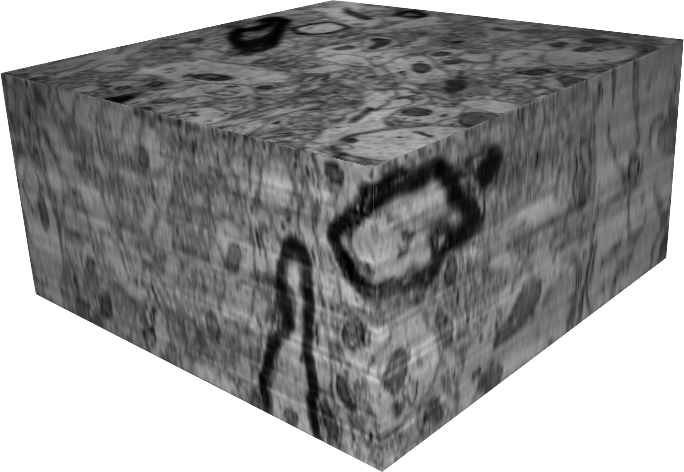
\includegraphics[height=.80\textwidth, width=\textwidth,keepaspectratio]{figures/intro/em_im.png}
	\end{subfigure}
	\hfill
	\begin{subfigure}[b]{\hwidth}
		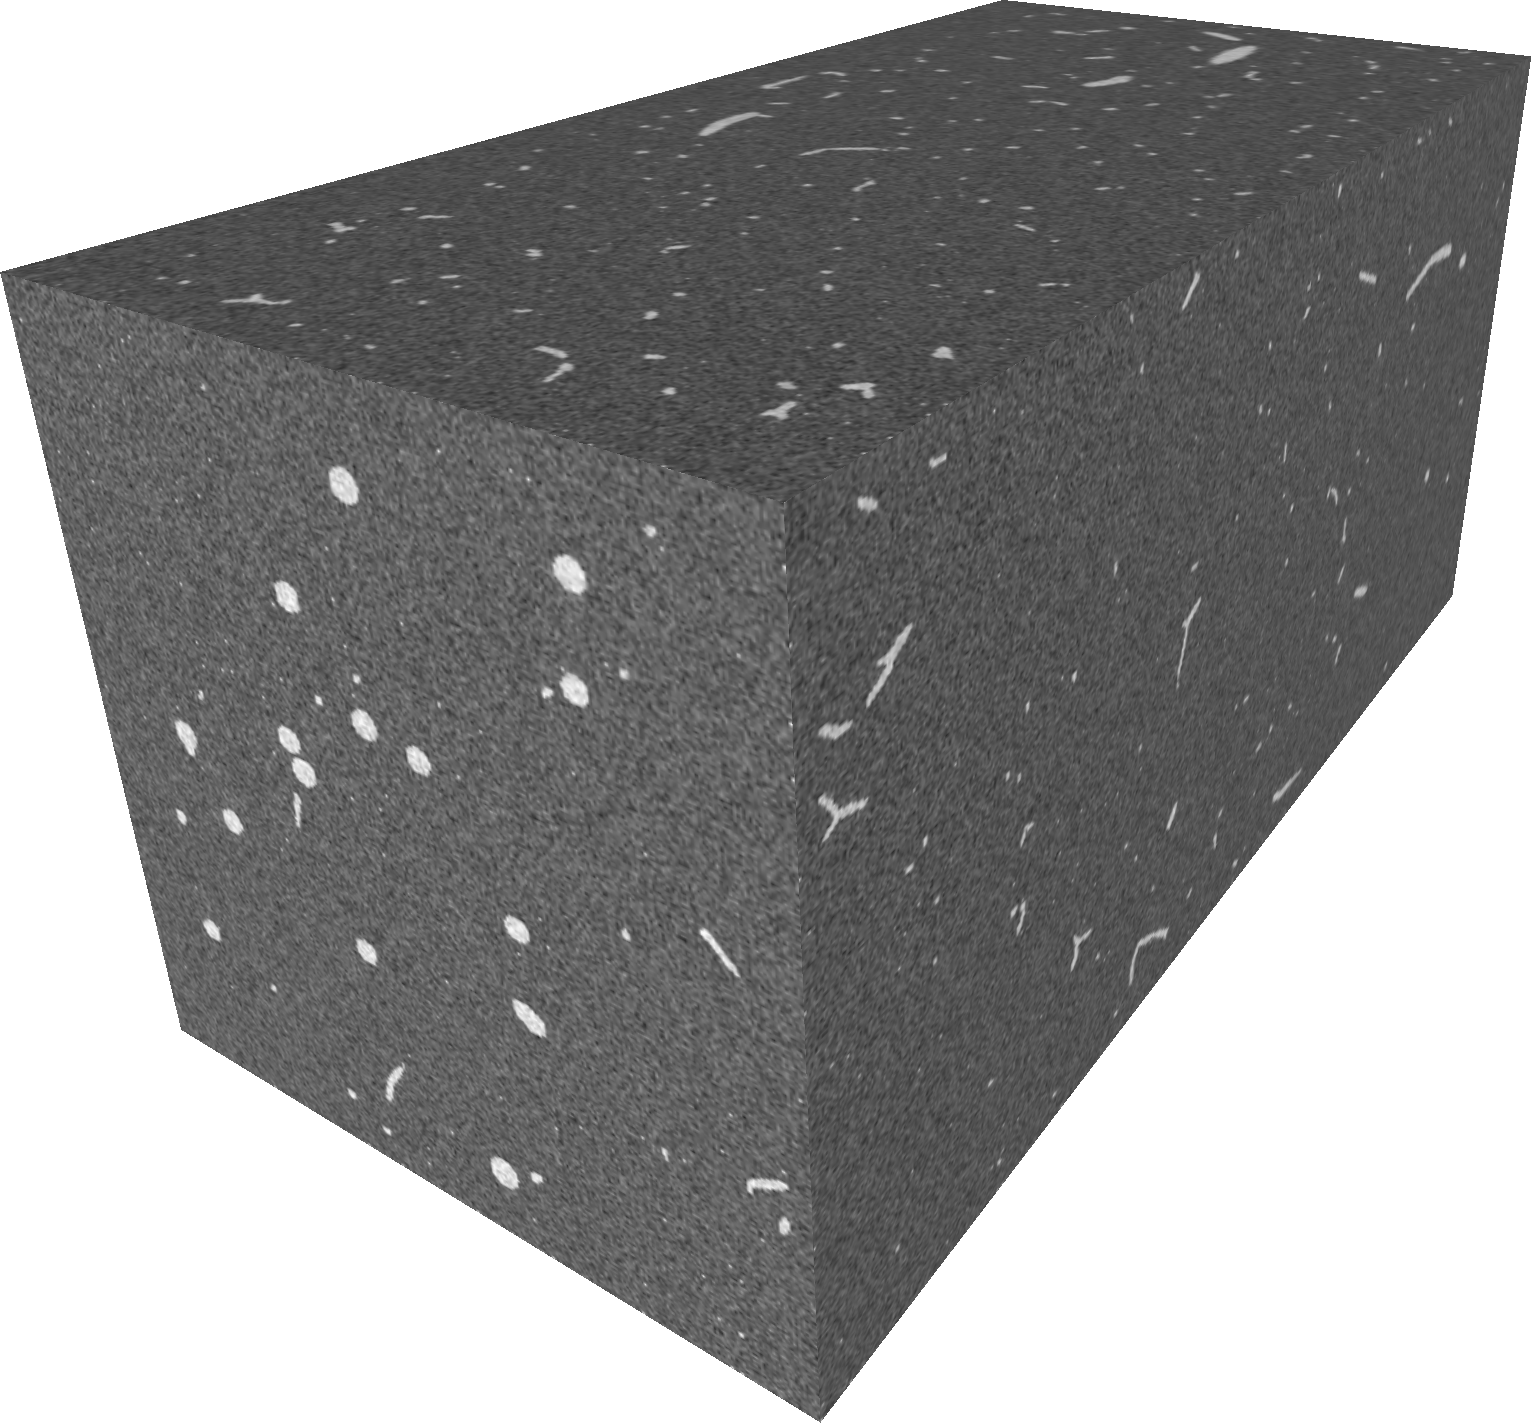
\includegraphics[height=.80\textwidth, width=\textwidth,keepaspectratio]{figures/intro/ct_im.png}
	\end{subfigure}
	\hfill
	\begin{subfigure}[b]{\hwidth}
		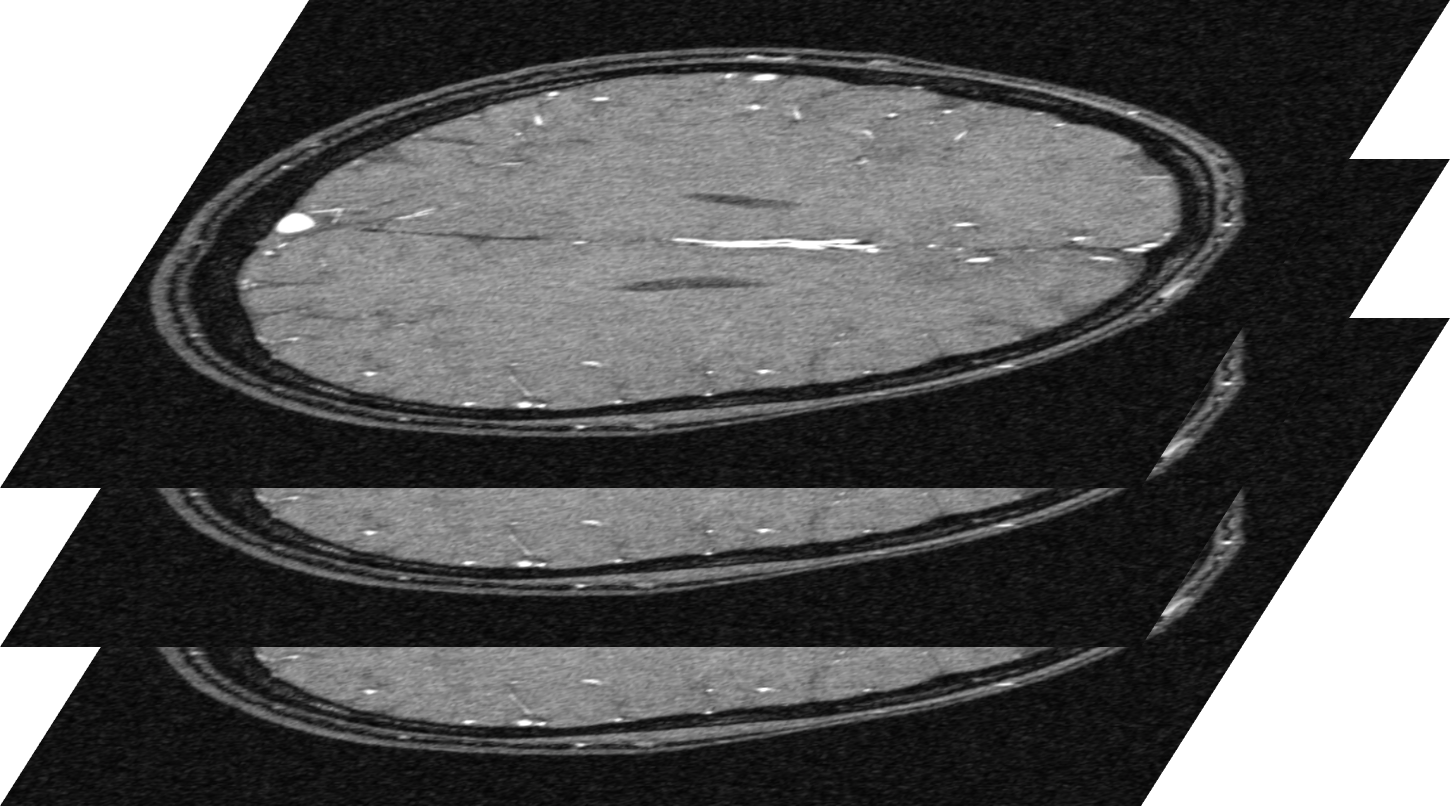
\includegraphics[height=.80\textwidth, width=\textwidth,keepaspectratio]{figures/intro/mri_im.png}
	\end{subfigure}\hfill\null\\
	\null\hfill
	\begin{subfigure}[b]{\hwidth}
		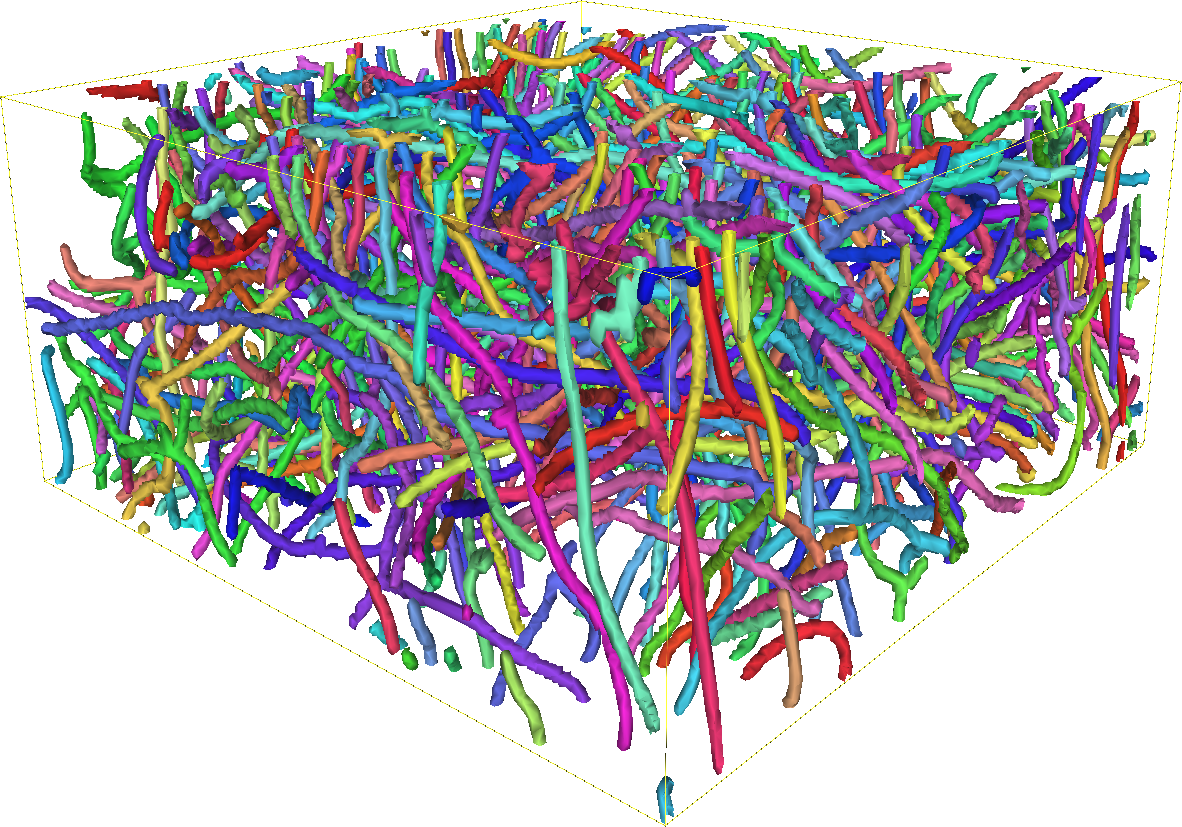
\includegraphics[height=.80\textwidth, width=\textwidth,keepaspectratio]{figures/intro/em_skel.png}
		\caption{\label{fig:intro_em}}
	\end{subfigure}
	\hfill
	\begin{subfigure}[b]{\hwidth}
		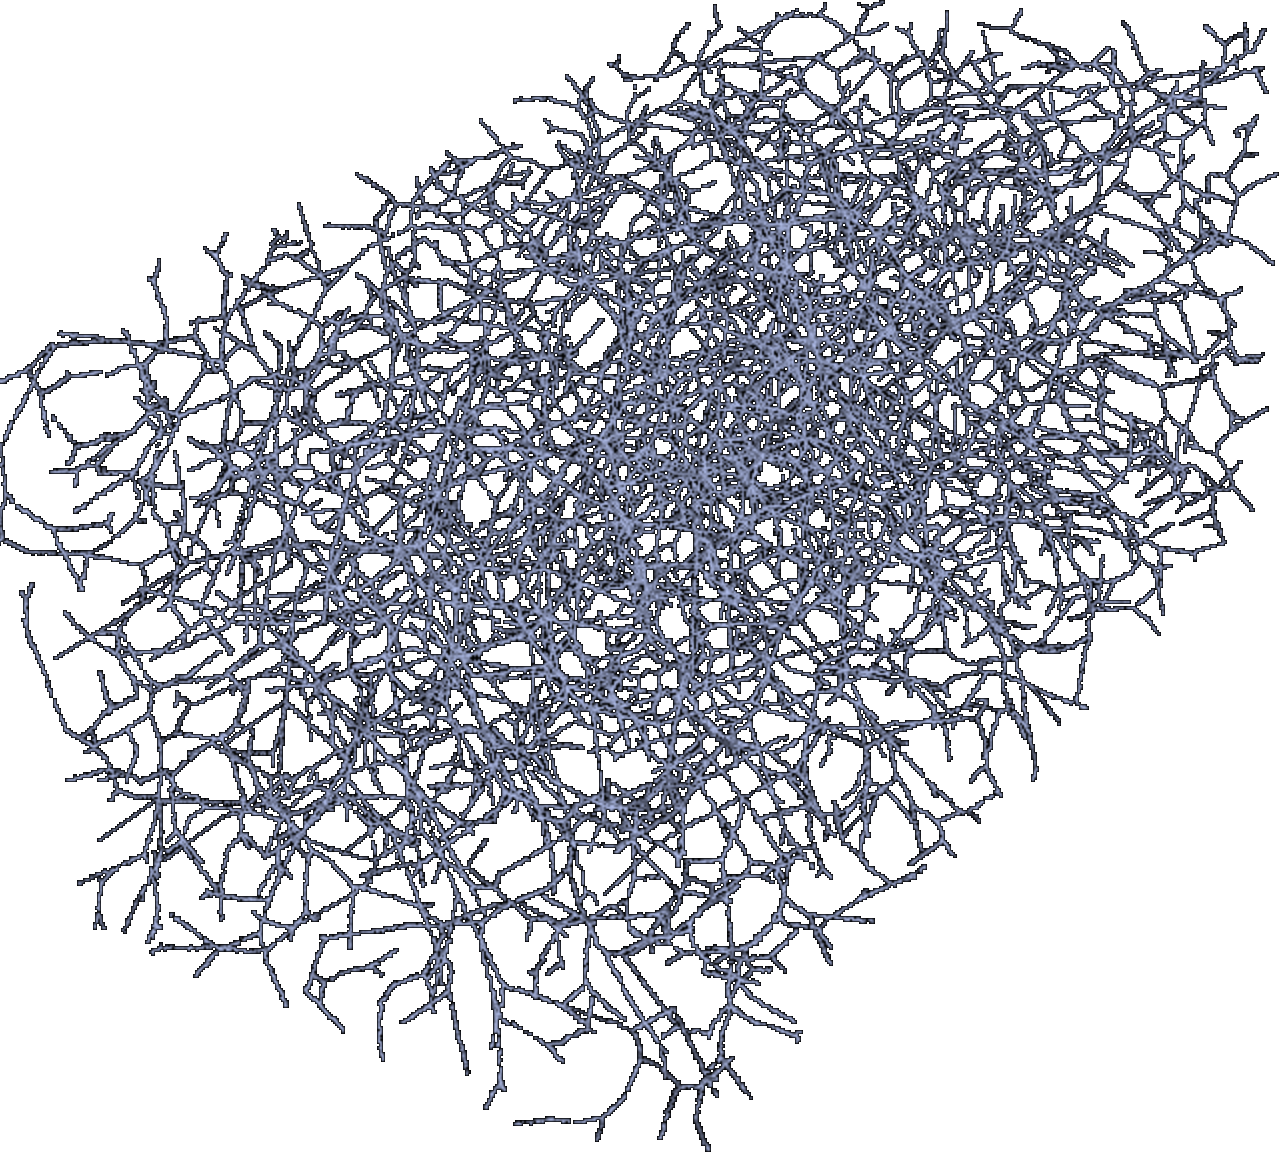
\includegraphics[height=.80\textwidth, width=\textwidth,keepaspectratio]{figures/intro/ct_skel.png}
		\caption{\label{fig:intro_ct}}
	\end{subfigure}
	\hfill
	\begin{subfigure}[b]{\hwidth}
		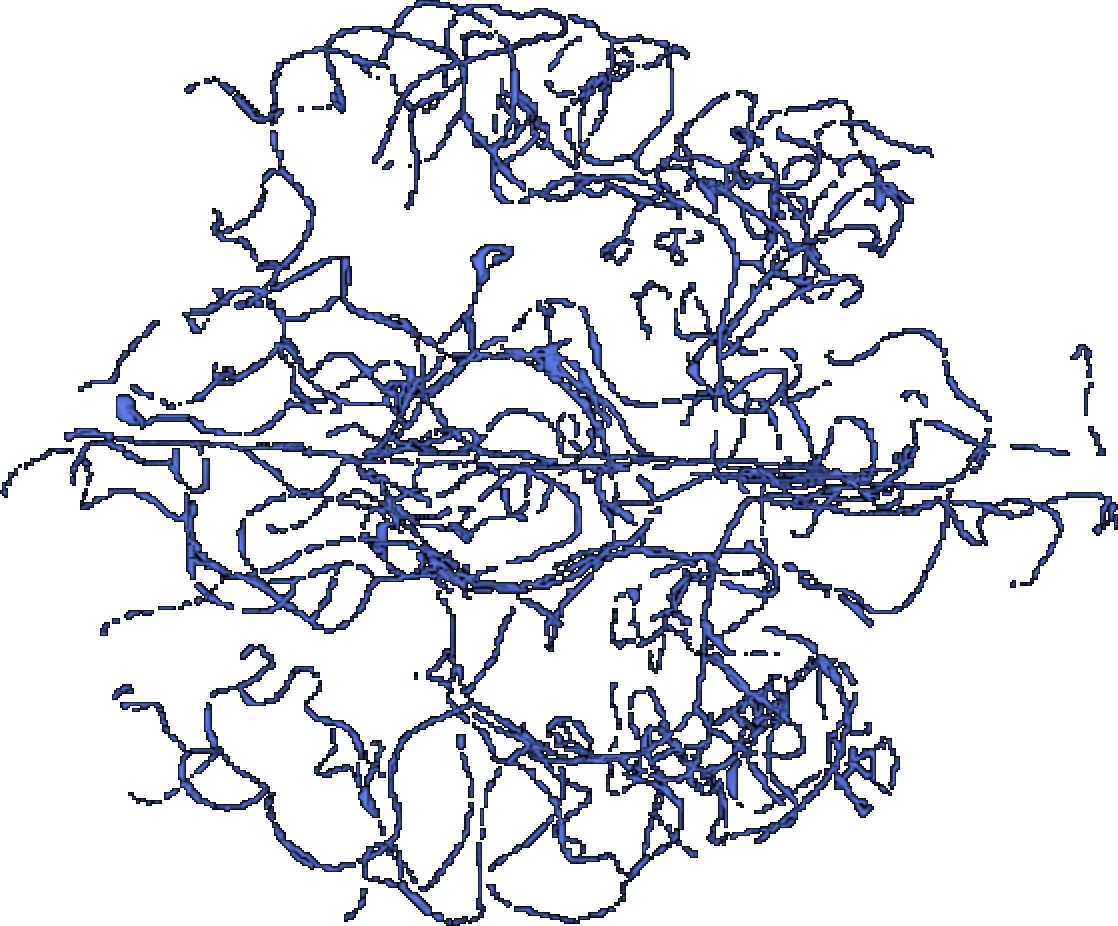
\includegraphics[height=.80\textwidth, width=\textwidth,keepaspectratio]{figures/intro/mri_skel.png}
		\caption{\label{fig:intro_mri}}
	\end{subfigure}
	\hfill\null
	\caption{3D Instance Skeleton Prediction. We predict (a) neuron skeletons from EM images, (b) blood vessel centerline from CT, and (c) brain vessel centerline from MRA}
	\label{fig:intro}
\end{figure}

\section{Motivation}
Instance skeleton extraction from volumetric data has numerous applications in the biomedical domain. For example, for neural circuit analysis~\cite{zheng2018complete} accurate wiring diagrams with skeletons and their synaptic connections can enable new insights into the workings of the brain and advance bio-inspired artificial intelligence. For clinical blood vessel analysis from CT images~\cite{Tetteh2018} we need accurate centerline and bifurcation prediction to quantify structural or flow patterns.

Another important application area is Connectomics \cite{Turaga2010, Funke2019, Kisuk2017} where although segmentation of electron microscopy(EM) images is a major step but it is not the final goal. It is important to find out interconnections between neurons, identify common neurons shapes~\cite{Zhao2014}, find geodesic distance between synapse connections and soma etc. Such analysis naturally calls in for skeletonization of neurons. A straight forward way is to skeletonize the predicted segmentations for which many algorithms already exist~\cite{TEASAR, Palagyi2014} but it is hard to obtain segmentation ground truth and state-of-the-art methods are either slow or produce results with many false merges and false splits. %Recently, skeletonization methods specially curated for EM images have also been proposed~\cite{Brian2019Skel}.

Apart from serving as a connectome analysis tool, skeletons could be instrumental in improving the segmentations itself. Since, they capture a global topology of segments they can be a indicator of false split and false merges in segmentation. A recent method by Matejek \etall~\cite{Brain2019} utilized skeleton end-points to identify false splits and merged them using skeleton curvature information.

Creating ground truth skeleton data is also easier than segmentation, dedicated tools like KNOSSOS~\cite{KNOSSOS} exist for easy labelling. Berning \etall~\cite{Berning2015} quotes skeleton labelling to be $25$ to $100$ times faster than segmentation labelling. It also proposes a semi-automatic segmentation method based on hand traced neurons. In another kind of neural images obtained from fluorescence confocal microscopy, neuron tracing methods \cite{Kayasandik2018} are being developed which is essentially skeletonization.

However, instance skeleton extraction is a challenging task. Due to complex 3D geometry. There can be false split and false merge errors among branches even for one instance, e.g. vascular tree. Besides, in brain electron microscopy (EM) images neurons are densely packed and their appearances have diverse textures which adds further complexity to the neural skeletonization process. 

There are two common approaches for instance skeleton extraction. One approach computes instance segmentation and applies thinning methods to obtain instance skeletons~\cite{Januszewski2018FFN}. The other approach computes semantic skeletons then uses connected components to distinguish different instances~\cite{Xu2019}.
In the first approach, obtaining satisfactory annotations is costly, it is much simpler to trace skeletons than delineate the detailed boundaries for object segmentation, \eg, neuron tracing in EM images. The second approach is prone to false merge errors when the skeletons are close to each other and false split errors when ambiguity exists in the image appearance.

In this work, we propose an end-to-end pipeline extracting instance-level skeletons for tubular structures. The pipeline includes three steps. 
\begin{itemize}
	\item First, we extend a 2D flux-based method~\cite{Wang2019} to predict 3D semantic skeletons. 
	\item Second, we create over-split skeleton instances. 
	\item In the last step, we connect the over-split instances using a recurrent tracking network.
\end{itemize}
We conduct quantitative evaluation on two public datasets from different biological domains (\autoref{fig:intro} (a, b)) and qualitative evaluation on a third dataset (\autoref{fig:intro} (c)). We show that the method learns high-quality intermediate representations for skeleton prediction. It also effectively overcomes the problem of split and merge errors suffered by most current end-to-end solutions. We compare our method with state-of-the-art methods~\cite{cciccek20163d,wang2019deep,Wang2019}.

\section{Related Work}
We review relevant skeleton extraction methods in 2D and 3D. We also review few instance segmentation methods for 3D EM images as it is similar to instance skeletonization problem.

\subsection{Skeleton Extraction} Earlier learning-based methods were developed by formulating skeleton extraction into a regression problem~\cite{Sironi2014} or leveraging the hypothesis that the contexts around skeletons are symmetric~\cite{Tsogkas2012}. Current state-of-the-art methods are mostly deep learning based which can be classified into two categories: 1) direct binary pixel classification~\cite{Tetteh2018,hifi2018,Liu2017}; 2) encoding skeletons in an intermediate representation~\cite{wang2019deep,Wang2019,sironi2015}. 
For the first approach, DeepVessel~\cite{Tetteh2018} proposed cross-hair filters from three intersecting 2-D filters to reduce training overhead while preserving 3D context information. Hi-Fi~\cite{hifi2018} proposes a new CNN architecture leveraging multi-scale features and bidirectional guidance to make binary predictions. In the second category, skeletons are encoded into intermediate representations like distance transform and context flux. The method in~\cite{wang2019deep} generates pseudo skeletons from learned nearest distance from any point to the tubular structure surface. DeepFlux~\cite{Wang2019} operates on natural images and learns relationships between image pixels and their closest skeletal points by flux field and recovers skeletons using magnitude and directions of predicted flux. It yields the best performance and therefore, we modify and extend DeepFlux and train our network to learn 3D flux as intermediate representation for skeletons. 


\subsection{Recurrent Methods for Instance Prediction}
% check related work for recurrent methods : https://arxiv.org/pdf/1708.02551.pdf
%For 2D natural images, recent works employ recurrent networks to sequentially generate instances. Stewart \textit{et al.} ~\cite{Stewart2016} train a long short-term memory (LSTM) network for end-to-end object detection with permutation-invariant loss and the Hungarian matching algorithm. Romera \textit{et al.}~\cite{Romera2016} improves upon it with a with convolutional LSTM model predicting binary mask for each instance.
%Recurrent methods are also prevalent in the applications involving 3D data.
We review few state-of-the-art methods which predicts curvilinear roads or its boundaries. This is in many ways similar to instance skeletonization. 

Recently proposed method by Liang \etall~\cite{Liang2019} predicts road boundaries using polyline representations by using a convolutional recurrent network, predicting one vertex at a time. An extension of their work, DAG-Mapper~\cite{Homayounfar2019}, takes into account road topology and predicts splits and merges too. Another recurrent road extraction method, RoadTracer~\cite{Bastani2018}, predicts road topology using a iterative search method guided by a convolutional neural network. 

Another related work, instance segmentation is also a similar problem like instance skeletonization, and a well known recurrent segmentation method used in the field of Connectomics \cite{Turaga2010, Funke2019, Kisuk2017} is flood-filling network (FFN)~\cite{Januszewski2018FFN}. It performs instance segmentation on 3D EM images by starting from a seed position and iteratively making predictions for overlapping sliding windows. Despite their outstanding performance, training a recurrent model is time-consuming. To overcome the above problem, instead of growing the entire structure step by step iteratively, we only apply the recurrent method on sparse locations which results in a more efficient algorithm.


\subsection{Error detection and Error Correction}
Instance skeletonization problem is similar to instance segmentation in a way that both can have false merges and splits. Therefore we can adopt ideas from segmentation methods in skeletonization to solve false merges and splits. 
In Connectomics~\cite{Turaga2010, Funke2019, Kisuk2017}, most connectomes reconstruction pipelines include an instance-level automatic error correction step. Zung \etall~\cite{Seung2017} trains classifiers to detect false splits and false merges for each object. They first train an error detection network to output an error map with the same size as the input image patch, centered at an voxel inside the object of interest. The second stage prunes object mask containing only merge errors obtained from superset of baseline object mask and detected error areas. However, the success of error correction largely depends on the accuracy of the error detection net. Another method by Matejek \etall~\cite{Brain2019} extract graphs from initial segmentations and exploit specific geometric and topological properties from underlying biological morphology to solve merge errors.


%\subsection{Flood Filling Network}
%All the previous discussed methods\textcolor{red}{cite segmentation papers}  were tuned and tested on relatively small scale data, but advancements in EM helped create larger and larger datasets reaching hundreds of Gigabytes, and the previous state-of-the-art couldn't catch up to produce acceptable results. But a recent method called Flood Filling Network (FFN)~\cite{Januszewski2018FFN} from Google was able to produce acceptable results for the first time on volumes of approx size $10K*10K*6K$ voxels.
%Their method segments one object at a time, growing its mask sequentially, until it traces the entire object. Initially a small seed is marked inside a segment, and a mask is predicted using a Deep Net for that single segment in a small field of view around that seed, further seed points are found inside the predicted mask by jumping a fixed step size in all possible directions.
%But similar to previous approaches neither can this method predict a mask completely accurately in one-shot. So, multiple iterations are run at different scales and seeding order to create a over-segmentation and then an extensive agglomeration step is performed using the same model.
%It is interesting to note that while this method is the state-of-the-art in connectomics, but apparently no other lab than Google has been able to use it for any large dataset. One reason being, with just $1000$ P100 GPUs it needs $16$ hours to run inference on the large volume\cite{Januszewski2017FFN}. So, currently its hard to put forth FFN as a general tool for Neuroscientists and a urgent need remains to create a segmentation tool which is feasible and easy to use.